\documentclass{my_paper}
\usepackage{ctex}
\usepackage[textwidth=444bp,vmargin=2.5cm]{geometry}%设置页边距
\usepackage{array} %主要是增加列样式选项
\usepackage[dvipsnames]{xcolor}%颜色宏包
\usepackage{graphicx}%图片宏包
\usepackage{amsmath}%公式宏包
\usepackage[T1]{fontenc}    
\usepackage{newtxtext, newtxmath}  %两种使用Times New Roman 字体的方法
\usepackage{subfigure}
\usepackage{tabularx, booktabs} %% Load packages that you use
\usepackage{multirow} %跨行处理
\usepackage{rotating}%横向表格
\usepackage{diagbox}%斜线划分表头

\usepackage { gensymb }
% 打°符号\degree
\usepackage{framed}
\usepackage{listings}
% 代码
\usepackage{color} %red, green, blue, yellow, cyan, magenta, black, white
\usepackage[numbered,framed]{matlab-prettifier}%matlab 代码高亮
\usepackage{mdframed}%另一个边框
% matlab代码样式,使用方法为:
% \lstinputlisting[style=Matlab-editor,linewidth=\textwidth]{code.m}
% 或:
% \begin{lstlisting}[style=matlab-prettifier]
%     %code
% \end{lstlisting}
\renewenvironment{framed}[1][\hsize]
  {\MakeFramed{\hsize#1\advance\hsize-\width \FrameRestore}}%
  {\endMakeFramed}
%   修正framed环境,使之可以变长,用法:
%   \begin{framed}[1.2/textwidth]...

\usepackage{hologo}
\usepackage{gbt7714}
\bibliographystyle{gbt7714-numerical}
% 采用国标参考文献引用
\newcommand{\lunwenbiaoti}{\fontsize{15.75pt}{0}\heiti 基于PID自动控制的暖气房屋控温模型}
\newcommand{\zhaiyao}{\fontsize{14pt}{0}\heiti 摘要}
    
\begin{document}

\lstdefinestyle{python_style}{
 columns=fixed,
 numbers=left,                                        % 在左侧显示行号
 numberstyle=\tiny\color{gray},                       % 设定行号格式
 frame=trbl,                                        % 单线背景边框
 breaklines=true,                                     % 设定LaTeX对过长的代码行进行自动换行
 keywordstyle=\color[RGB]{40,40,255},                 % 设定关键字颜色
 numberstyle=\footnotesize\color{darkgray},
 commentstyle=\it\color[RGB]{0,96,96},                % 设置代码注释的格式
 stringstyle=\rmfamily\slshape\color[RGB]{128,0,0},   % 设置字符串格式
 showstringspaces=false,                              % 不显示字符串中的空格
 language=python,                                        % 设置语言
 basicstyle=\linespread{1.0}\fontsize{10bp}{10bp}\selectfont\ttfamily,                      % 字体字号
 %lineskip=10bp,
 %baselinestretch=1,
}
\newpage
\begin{center}
\lunwenbiaoti

\vspace{2ex}
\zhaiyao
\end{center}

摘要

\begin{guanjianci}
 元胞自动机 \quad 边缘检测 \quad 形状匹配
\end{guanjianci}

%----------- 正文 ----------
%----------- 一、问题重述 ----------
\newpage
\section{一、问题重述}

\subsection{问题背景}

我国具有悠久的玻璃制作历史,玻璃是丝绸之路历史的重要物证,在考古工作中,需要对玻璃的成分进行分析,并对其种类进行鉴别。

玻璃以石英砂(主要成分为$SiO_2$)作为主要原料,在制造的过程中为了降低熔点,添加不同的助熔剂进行炼制,并加入氧化钙等作为稳定剂。根据所加入助熔剂的不同,玻璃化学成分产生差异,这使得古代玻璃产生了不同的种类。例如添加铅矿石作为助熔剂的玻璃含有较高的氧化钡和氧化铅含量,常被称作铅钡玻璃;添加草木灰等作为助熔剂的玻璃,具有较高的钾含量,被称作是钾玻璃。

古代玻璃经由漫长的埋藏过程而导致风化。风化的本质是玻璃与外界环境之间产生了元素交换,导致成分发生变化。风化过程的程度不同,导致玻璃的成分,颜色发生较大变化,给考古工作带来了一定困难。
我们需要利用古代玻璃采样的化学检测数据,探究风化与物质成分的变化关系,以及分类标准与成分之间的相关关系。

\subsection{问题重述}
经过分析整理,我们需要解决以下问题:
\begin{enumerate}
    \item 分析表面风化同玻璃类型、纹饰和颜色之间的关系进行分析,并就类别分析其风化前后的化学含量统计规律,最后根据风化点的检测数据预测未风化前的物质含量。
    \item 分析高钾玻璃和铅钡玻璃之间的类别划分规律,对每个类别选择合适的指标进行亚类的划分,给出划分的结果,并对结果进行敏感性分析。
    \item 对所给附件中未知类别的玻璃文物化学成分进行分析,鉴定所属类别,并对分类结果进行敏感性分析。
    \item 针对不同类别的玻璃文物样品,在不同的化学成分中分析关联关系,对这一关系的差异程度进行分析。
\end{enumerate}
\section{二、问题分析}
\subsection{问题一的分析}

为了解决第一小问,我们首先对原始数据进行清洗,对不满足成分性要求的数据进行剔除。为了分析便面风化与类型,纹饰,颜色之间的关系,考虑使用皮尔逊的拟合优度检验法\cite{1}或是方差分析\cite{2}等方法,分析三个因素与风化之间的关系。

\subsection{问题二的分析}

分析

\subsection{问题三的分析}


%----------- 三、模型假设 ----------
\section{三、模型假设}
%使用代码片段:、jiashe%
\begin{enumerate}
    \item 
    
    \textbf{原因:}


\end{enumerate}

%----------- 四、符号说明 ----------
\section{四、名词解释与符号说明}
%使用三线表格最好~
\subsection{名词解释}
\begin{enumerate}
    % 名词:、mingci
    \item \textbf{dada}
    
    dsadw
    
    \item \textbf{dsadc}
    
    dasdsas

    
\end{enumerate}
\subsection{符号说明}
以下是本文使用的符号以及含义:
\begin{table}[h]%htbp表示的意思是latex会尽量满足排在前面的浮动格式,就是h-t-b-p这个顺序,让排版的效果尽量好。
    \centering
    \begin{tabular}{p{2.0cm}<{\centering}p{9.0cm}<{\centering}p{2.0cm}<{\centering}}
 %指定单元格宽度, 并且水平居中。
    \hline
    符号 & 说明 & 单位 \\ %换行 
    \hline
    $L_0$ & 仓库长度 &  $m$\\
    
    \hline
    \end{tabular}
\end{table}

%----------- 五、模型的建立与求解 ----------
\section{五、模型的建立与求解}

以下将对提出的四个问题进行建模求解。
\subsection{数据清洗与可视化分析}
在这一部分,我们进行了一些数据预处理工作。首先对剔除不满足要求的数据,随后对缺失的数据进行填补,最后将数据进行分析统计,以更好的进行建模活动。

\subsubsection{剔除异常数据}
根据题目信息,需要对不满足成分性的数据进行剔除。成分性的定义为各个成分之间的加和应该是等于$ 100\% $,但是由于种种因素这一性质不能达到。规定各个组分的加和处于$85\%\sim 105\%$之间的数据作为有效数据。对表单2中的69条数据进行统计,得到图(\ref{51})所示的结果。
\begin {figure}[h]
\centering % 居中显示
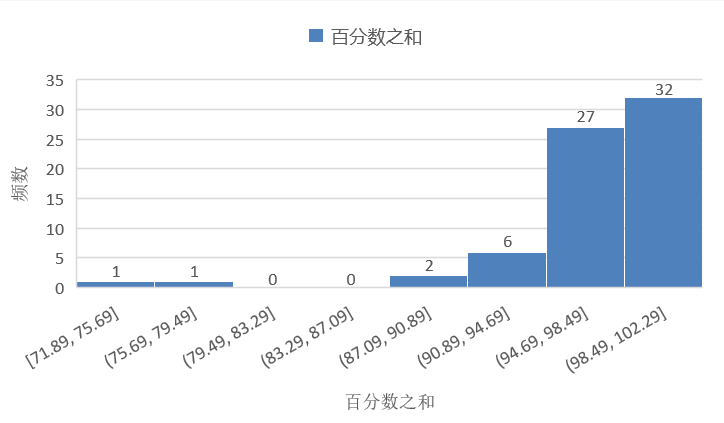
\includegraphics[width=0.7\textwidth]{51.png}
\caption{附件二各采样点成分的求和} % 标题
\label{51}
\end {figure}

可见数据总体分布在$87.09\%\sim 102.29\%$这一区间中,只有两条记录不能满足成分性,分别是17号采样点$71.89\%$以及15号采样点$79.47\%$,将其剔除。

\subsubsection{数据填补}
在58份样本数据中分别说明了其编号、纹饰、类型、颜色与风化程度五项数据,其中颜色一项有四条缺失,分别位于编号 19 、40、 48和58处。为了便于后续的分析处理,将缺失项用“未知”填补,补全了数据缺口。

\subsubsection{可视化分析}
为了便于后续的分析处理,我们对数据进行可视化分析。为了判断类别分布的规律,首先对文物样本在各个指标的分布情况进行分析,得到图(\ref{513})所示的结果。
\begin{figure}[htbp]
    \centering  %居中
    \subfigure[纹饰分布]{   %第一张子图
    \begin{minipage}{0.35\textwidth}%大小总和超过textwidth则自动换行
    \centering    %子图居中
    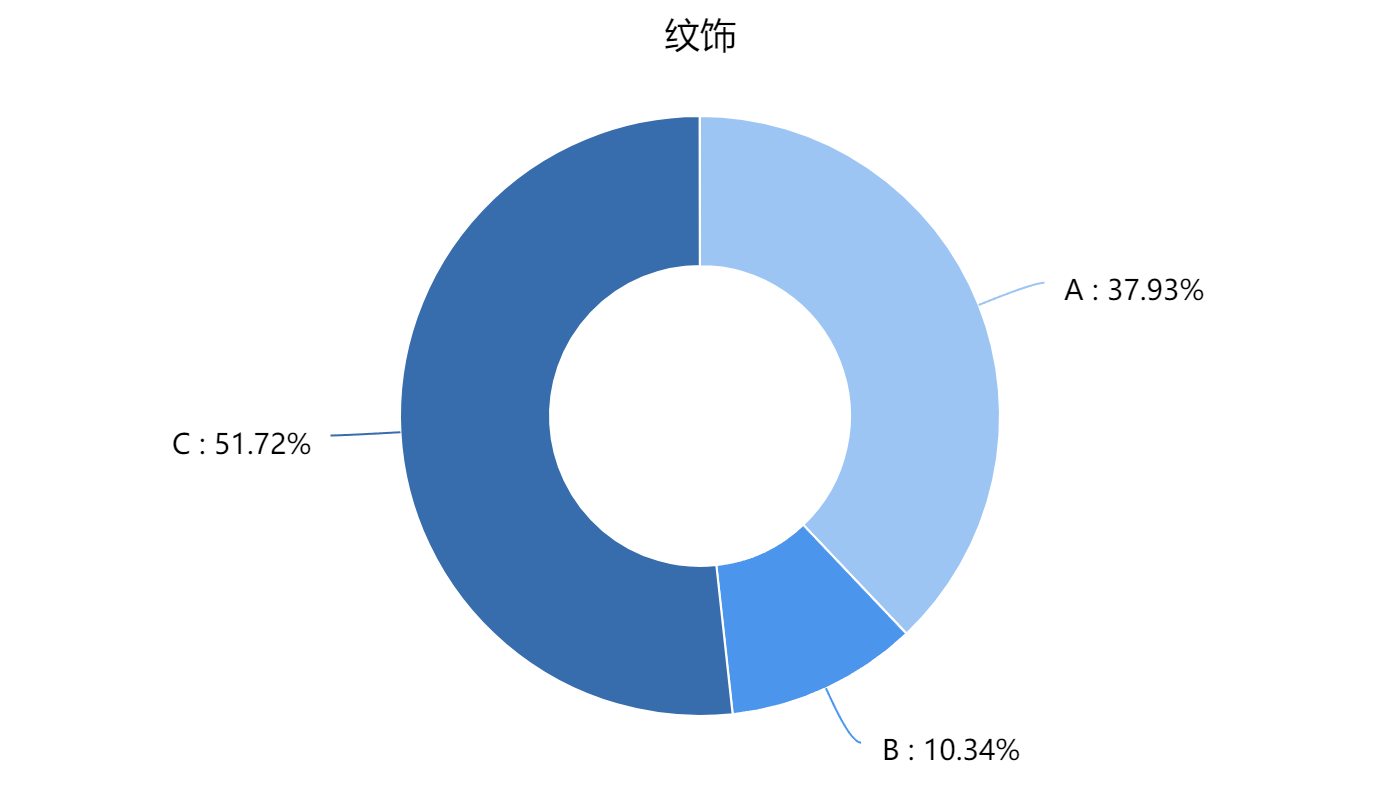
\includegraphics[width=\textwidth]{513ws.png}  %设置图片的输出大小倍数,这里是0.5倍大小输出
    \end{minipage}
    }
    \subfigure[类型分布]{   %子图
    \begin{minipage}{0.35\textwidth}%大小总和超过textwidth则自动换行
    \centering    %子图居中
    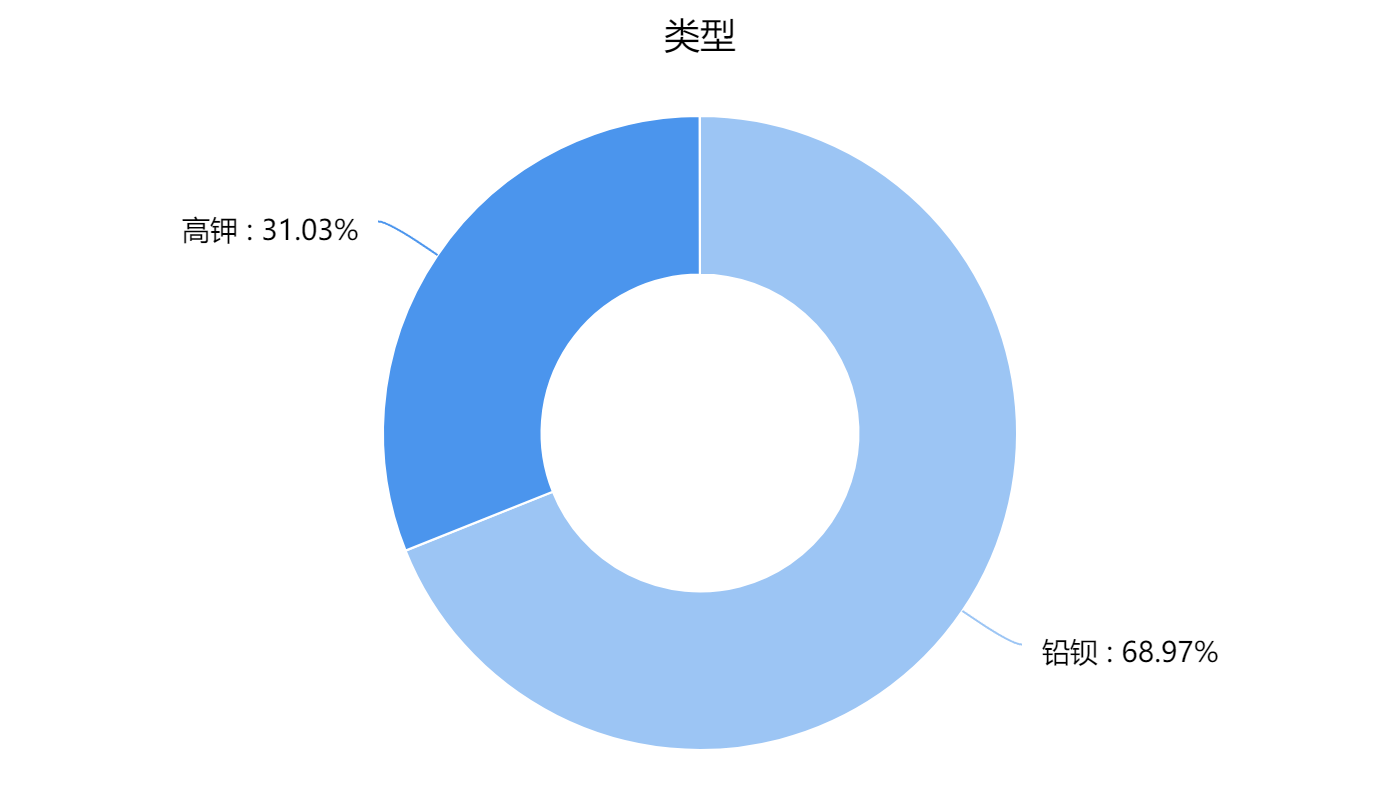
\includegraphics[width=\textwidth]{513lx.png}  %设置图片的输出大小倍数,这里是0.5倍大小输出
    \end{minipage}
    }\\
    \subfigure[颜色分布]{ %第二张子图
    \begin{minipage}{0.5\textwidth}
    \centering    %子图居中
    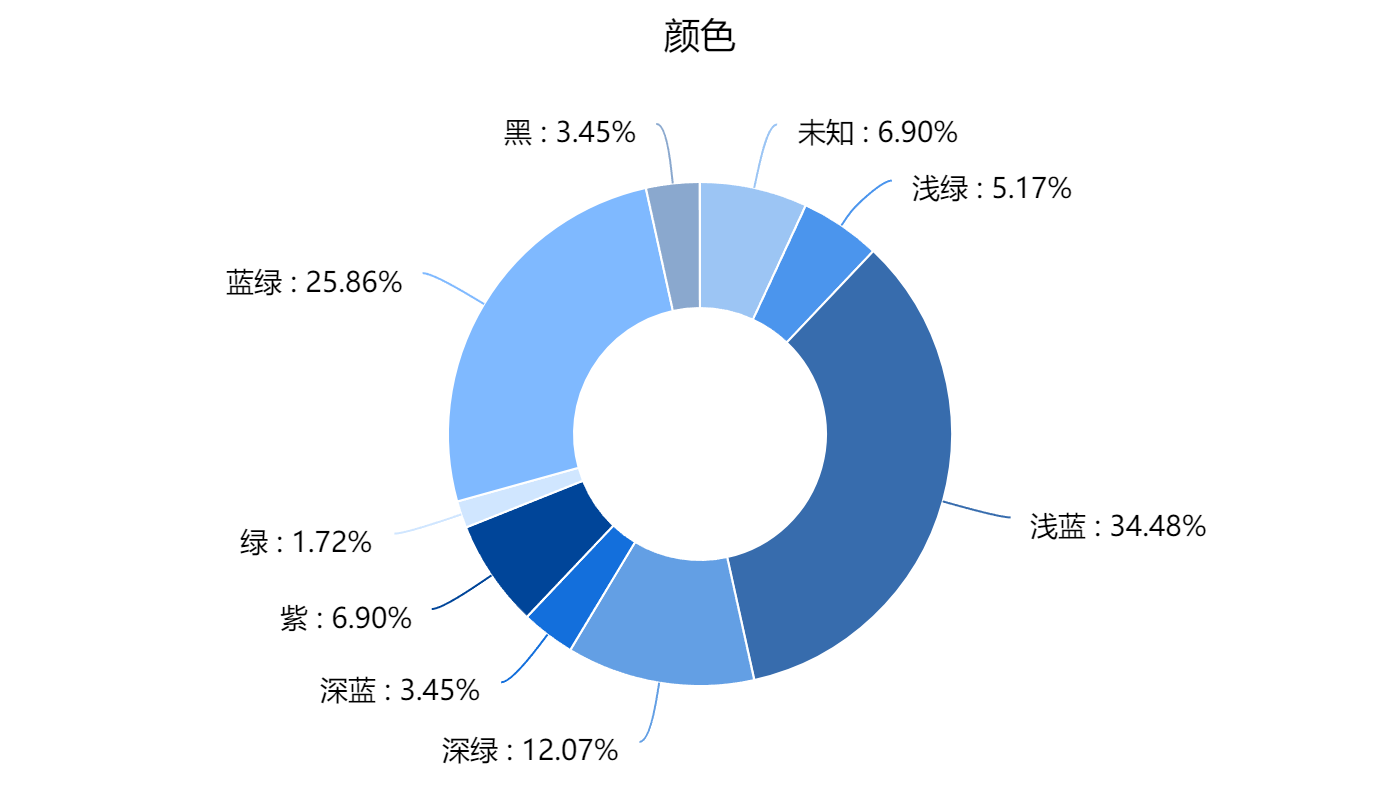
\includegraphics[width=\textwidth]{513ys.png}%以pic.jpg的0.5倍大小输出
    \end{minipage}
    }
    \caption{玻璃样本基本信息的分布情况}    %大图名称
    \label{513}    %图片引用标记
\end{figure}
可见古代玻璃样本以C类型的纹饰为主,其次是A纹饰,B纹饰的占比最小,仅占$10.34\%$。在类型分布上,铅钡玻璃的占比超过了三分之二,成为数量较多的一类。在颜色分布上,颜色以蓝、绿为主,可能是由于其中的$Fe^{3+}$,$ Cu^{2+} $等离子的存在而显色\cite{3}。其中颜色由显现出不同的深浅,可能代表显色物质的组合以及浓度差异。
\subsection{古代玻璃风化预测模型}
在本部分,我们首先对古代玻璃的种类、纹饰和颜色,同风化的相关关系进行分析,利用多种方法分析出与风化关系密切的因素。随后我们就玻璃种类和风化与否来划分成分含量指标,给出成分的统计规律,随后建立模型,对古代玻璃的未风化前的元素含量做出预测。

\subsubsection{古代玻璃各指标相关性分析}
为了探究古代玻璃的纹饰种类、类型与颜色等因素的差异对于玻璃风化程度的影响,对这三个因素进行相关性分析。我们首先使用方差分析\cite{2}检验相关性。下面以检验纹饰同风化之间的关系叙述计算过程。

我们若将纹饰视作考察的因素,那么不同的纹饰$\{A,B,C\}$则可以视为$r$个不同的水平,这里$r=3$,若用附件所给58个玻璃样本数据进行分析,在各个样本独立同分布的条件下,记录第$k$种纹饰中第$i$个样本的风化程度为$X_{ik}$,每种纹饰的样本数量为$n_A,n_B,n_C$。根据上述信息,可以得到水平项离差平方和(SSA)、误差项离差平方和(SSE)的统计量$SS_A$与$SS_E$:
\begin{equation}
    \mathrm{SS}_{\mathrm{A}}=\sum_{i=1}^{r} \sum_{j=1}^{n_{i}}\left(\bar{X_{i}}-\bar{X}\right)^{2}=\sum_{i=1}^{r} n_{i}\left(\bar{X_{i}}-\bar{X}\right)^{2} 
\label{ssa}
\end{equation}
\begin{equation}
    \mathrm{SS}_{\mathrm{E}}=\sum_{i=1}^{r} \sum_{j=1}^{n_{i}}\left(X_{i j}-\bar{X_{i}}\right)^{2}
    \label{sse}
\end{equation}


方差分析的基本思想是通过水平项离差平方和(SSA)、误差项离差平方和(SSE)的统计量判断假设$H_0$:$\mu_1=\mu_2=\cdots=\mu_r$是否成立。这里的$\mu$代表风化程度的均值。当上述假设成立时满足下式:

$$\frac{\mathrm{SS}_{\mathrm{A}}}{\sigma^{2}} \sim \chi^{2}(r-1), \quad \frac{\mathrm{SS}_{\mathrm{E}}}{\sigma^{2}} \sim \chi^{2}(n-r)$$

样本的方差是未知的变量,构造检验量$F$进行处理,将其消去,得到下式:
\begin{equation}
    F=\frac{\mathrm{SS}_{\mathrm{A}} / \mathrm{df}_{\mathrm{A}}}{\mathrm{SS}_{\mathrm{E}} / \mathrm{df}_{\mathrm{E}}}=\frac{\mathrm{MS}_{\mathrm{A}}}{\mathrm{MS}_{\mathrm{E}}} \sim F(r-1, n-r)
\label{F}
\end{equation}

其中$MS_A$与$MS_E$称作是均方和,以$F$的显著性大小来检验纹饰种类同风化情况之间的关联程度。而对于颜色和类型的水平与风化程度的分析方面,我们可以使用相似的方法进行分析。下面将给出三个指标相关性分析的结果。

经过计算,三个因素的重要参数罗列在表(\ref{fc})中。
\begin{table}[t]
\centering
\caption{根据类型 、纹饰和颜色的方差分析结果}
\begin{tabular}{c|ccc}
\toprule
\diagbox{指标}{因素}& 类型     & 纹饰      & 颜色     \\\midrule
$SS_A$ & 1.669  & 1.2023  & 2.288  \\
$SS_E$ & 12.4   & 12.8667 & 11.781 \\
$MS_A$ & 1.669  & 0.6011  & 0.2542 \\
$MS_E$ & 0.2214 & 0.2339  & 0.2454 \\
$F$    & 7.5373 & 2.5697  & 1.0358 \\
\bottomrule
  \end{tabular}
\label{fc}
  \end{table}

  查表\cite{4}可知,类型 、纹饰和颜色三个因素所得$F$值在如下对应范围内,对三个因素,我们分别给定假设检验水平
  \begin{align}
    F_{0.01}(1,40)=
  \end{align}
\section{六、敏感性分析}
\section{七、模型的评价}

\subsection{模型的优点}
\begin{enumerate}
    \item 采用

\end{enumerate}

\subsection{模型的缺点}
\begin{itemize}
    \item 利用较

\end{itemize}

%----------- 参考文献 ----------
\newpage
\begin{center}
\bibliography{r} %调出LaTeX生成参考文献列表
\end{center}

%----------- 附录 ----------
\newpage
\section{附件}
\textbf{附件清单:}
\renewcommand\theenumi{\roman{enumi}}
% 规定数字格式为罗马数字
\renewcommand\labelenumi{\textbf{附录\theenumi}}
% 规定是附录某某
\begin{itemize}
    \item da 
    % \lstinputlisting[style=Matlab-editor,linewidth=\textwidth]{code.m}
\end{itemize}



% \lstinputlisting[style=Matlab-editor,linewidth=\textwidth]{code.m}




\end{document}